
\documentclass{ppgeesa}

%%%%%%%%%%%%%%%%%%%%%%%%%%%%%%%%%%%%%%%%%%%%%%%%%%%%%%%%%%%%%%%%%%%%%%%%%%%%%%%%%%%%%%%%%%%%%%%%%%%%%%%%%%%%%%%%%

\usepackage[latin1]{inputenc}
\usepackage{graphicx}
\usepackage{hyperref}
\usepackage{tikz}
\usepackage{amsmath}
\usepackage{listings}

\lstset{stepnumber=2, frame=single,tabsize=2, breaklines=true, basicstyle=\footnotesize}

\hypersetup{
	colorlinks,
	debug=true,
	linkcolor=black,  %%% cor do tableofcontents, \ref, \footnote, etc
	citecolor=red,  %%% cor do \cite
	urlcolor=blue,   %%% cor do \url e \href
	bookmarksopen=true,
	pdftitle={Filtro de Kalman},
	pdfauthor={Tassiano Neuhaus},
	pdfsubject={Sistemas de controle multivari�veis},
	pdfkeywords={Controle}
	%pdfpagemode=FullScreen
}

%%%%%%%%%%%%%%%%%%%%%%%%%%%%%%%%%%%%%%%%%%%%%%%%%%%%%%%%%%%%%%%%%%%%%%%%%%%%%%%%%%%%%%%%%%%%%%%%%%%%%%%%%%%%%%%%%


\begin{document}

\title{Filtro de Kalman, LQG e LQR em tempo discreto}

\author{Tassiano Neuhaus\\
{\small Universidade Federal do Rio Grande do Sul - Departamento de Engenharia El�trica\\Av. Osvaldo Aranha, 103 - Bairro Bom Fim CEP: 90035-190 - Porto Alegre - RS - Brazil}\\
}%\thanks{Tassiano Neuhaus, tassianors@gmail.com, Tel +55-51-91760154}}

\maketitle
\thispagestyle{empty}\pagestyle{empty}

\begin{abstract}
Este trabalho apresenta a formulac�o do filtro de Kalman e algumas de suas aplica��es.

Apresenta tamb�m a o problema de Linear-Quadratic Regulator (LQR) e Linear-Quadratic 
Gausian (LQG) para tempo discreto.
\end{abstract}

\begin{IEEEkeywords}
Filtro de Kalman, LQG, LQR.
\end{IEEEkeywords}

%===============================================================================
\section{Introdu��o}

Neste Trabalho ser� abordado aspectos da modelagem e utiliza��o do filtro 
de Kalman  (Sec. \ref{sec:kalman_filter}), suas aplica��es para o ramo da
engenharia (Sec. \ref{sec:applications}) e sua modelagem para o tempo discreto,
ser� apresentado uma breve descri��o das vantagens que o filtro possui e sua 
grande robustez para sistema sujeitos a perturba��es, ruidos ou imprecis�o na 
sua modelagem.

Ser� abordado o problema de LQG e LQR para o sistema de tempo discreto
(Sec. \ref{sec:lqg_lqr}), ser� apresentado tamb�m o principio da separa��o para
a resolu��o do problema do filtro de Kalman.

Ao fim ser� apresentado as conclus�es (Sec. \ref{sec:concl}) obtidas com o
trabalho desenvolvido.


\section{Filtro de Kalman}
\label{sec:kalman_filter}
%===============================================================================
\subsection{Hist�ria}

Em 1960 Rudolph Emil Kalman publicou um famoso artigo \cite{kalman60} descrevendo
um processo recursivo para solucionar problemas lineares relacionados � filtragem
de dados discretos. Sua pesquisa proporcionou contribui��es relevantes ajudando
a estabelecer bases te�ricas s�lidas em v�rias �reas da engenharia de sistemas. Em
1960-1961 Kalman desenvolveu, com colabora��o de Richard S. Bucy, a vers�o
em tempo cont�nuo do filtro de Kalman, que se tornou conhecida como o filtro de
Kalman-Bucy \cite{kalman_bucy}. Com o avan�o computacional, o filtro de Kalman e
suas extens�es a problemas n�o lineares representam o produto mais largamente
utilizado dentro da moderna teoria de controle.

%===============================================================================
\subsection{O Filtro} 

O filtro de Kalman assume que a fun��o densidade de probabilidade em cada
instante de tempo segue uma distribui��o Gaussiana. Este filtro permite a
estimativa do estado de um sistema de forma a minimizar o quadrado da
m�dia do erro \cite{welch_bishop}, tratando-se de uma solu��o �tima para o seguimento,
caso sejam satisfeitas algumas restri��es: se o ru�do tiver uma distribui��o
Gaussiana de par�metros conhecidos e se a transi��o de estados representada
pelo modelo do sistema for linear \cite{welch_bishop} \cite{Arulampalam}.

O Filtro de Kalman � bastante poderoso e vers�til em diversos aspectos: ele 
suporta estima��es do passado, presente e at� mesmo futuros estados do sistema, 
mesmo quando o modelo do sistema n�o � totalmente conhecido.\cite{welch_bishop}

%===============================================================================
\subsubsection{Filtro de Kalman Discreto}

O Filtro de Kalman foi altamente difundido por sua robustez e facilidade de implementa��o
do algoritmo proposto. Desta forma sistemas computacionais podem, de forma bem
eficiente, utilizar o filtro e expandir a sua utiliza��o.

O processo a ser estimado � o descrito em (\ref{eq:sis_disc}) com $x \subset \Re^{n}$ e
com a sa�da mensur�vel descrita por (\ref{eq:sis_disc_out}) onde $z \subset \Re^{m}$.

\begin{equation}
x_k = Ax_{k-1} +Bu_{k-1}+w_{k-1}
\label{eq:sis_disc}
\end{equation}

\begin{equation}
z_k = Hx_k + \nu_k
\label{eq:sis_disc_out}
\end{equation}

As origens computacionais do filtro:

Define-se $\hat{x}_{k}^{-} \in \Re^n$ como sendo o estado {\it{a priori}} estimado para
um $k$ definido, bastando para isso o conhecimento do estado anterior. Chama-se 
$\hat{x}_{k} \in \Re^n$ como sendo o estado {\it{a posteriori}}. Pode-se definir estados
pelas equa��es abaixo:

\begin{equation}
\begin{matrix}
e_{k}^{-} \equiv x_k - \hat{x}_{k}^{-} 
\\ e \\ 
e_{k} \equiv x_k - \hat{x}_{k}
\end{matrix}\nonumber
\end{equation}

Na Equa��o (\ref{eq:xk}) observa-se que o estado {\it{posteriori}} � uma combina��o 
linear do estado {\it{priori}} com um balanceamento entre a atual medida $z_k$ e a
predi��o $H \hat{x}_{k}^{-}$.

\begin{equation}
\hat{x}_k = \hat{x}_{k}^{-}+K(z_k -H\hat{x}_{k}^{-})
\label{eq:xk}
\end{equation}

O ganho $K$ � escolhido a fim de minimizar o erro da covari�ncia do estado 
{\it{posteriori}}. Um dos poss�veis valores que minimiza este crit�rio pode ser
observado em (\ref{eq:k_posteriori}).

\begin{equation}
K_k=P_{k}^{-}H'(HP_{k}^{-}H'+R)^{-1}
\label{eq:k_posteriori}
\end{equation}

%===============================================================================
\subsection{Algoritmo}

O filtro de Kalman utiliza realimenta��o para estimar os valores dos estados:
Ele estima o estado do processo em um determinado tempo e ent�o obt�m a realimenta��o 
o valor medido (podendo haver ruido). Desta forma o filtro pode ser dividido em duas
partes principais: Equa��es de tempo e equa��es de medida. As equa��es de tempo tem
como finalidade a proje��o (em quest�es de tempo) o estado atual e a covari�ncia 
para obter a {\it{priori}} estima��o para o pr�ximo passo. As equa��es de medida 
s�o respons�veis pela realimenta��o, adicionando algumas medidas ao estado {\it{a priori}} 
para obter um estado {\it{a posteriori}} mais acurado. Este procedimento pode ser observado
na Figura (\ref{fig:kalman_cicle}).

\begin{figure}[htbp]
	\center
	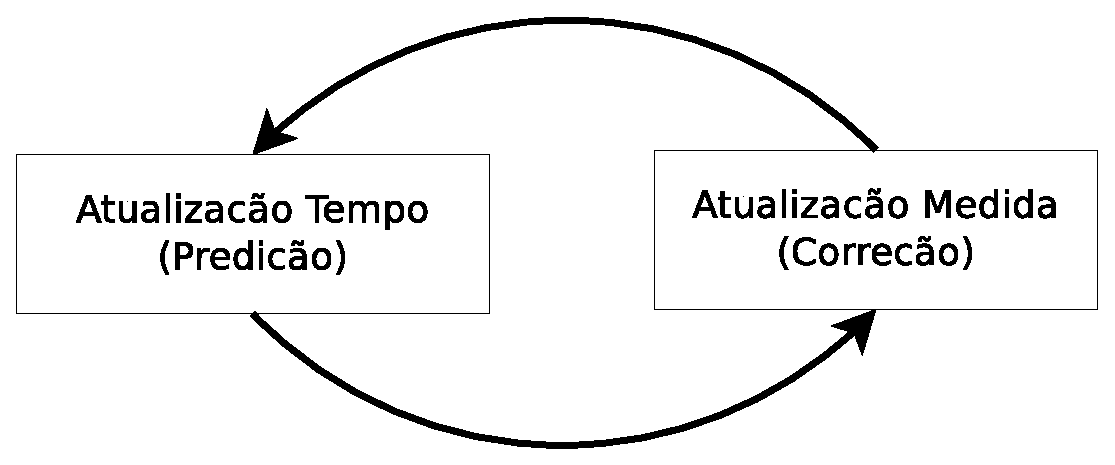
\includegraphics[width=0.60\columnwidth]{figures/kalman_alg.eps}
	\caption{Ciclo de funcionamento do filtro de Kalman. \cite{welch_bishop}}
	\label{fig:kalman_cicle}
\end{figure}

Nas Equa��es (\ref{eq:time_update1}) e (\ref{eq:time_update2}) podem ser observadas as 
equa��es referentes a etapa de Time Update e as equa��es de Measurement Update s�o apresentadas
em (\ref{eq:k_posteriori}), (\ref{eq:xk}) e (\ref{eq:measurement_update}).

\begin{equation}
	\hat{x}_{k}^{-}=A\hat{x}_{k-1} + Bu_{k-1}
	\label{eq:time_update1}
\end{equation}

\begin{equation}
	P_{k}^{-}=AP_{k-1}A'+Q
	\label{eq:time_update2}
\end{equation}

\begin{equation}
	P_k = (I - K_k H)P_k^{-}
	\label{eq:measurement_update}
\end{equation}

Na atual implementa��o do filtro a medida da covari�ncia do ruido ($R$) � algo fact�vel
na pratica pois � necess�rio medir o processo de qualquer forma. Desta forma algumas
medidas off-line s�o necess�rias para se conhecer esta covari�ncia do ruido.

A determina��o do ruido de covari�ncia do processo ($Q$) � geralmente mais dif�cil de ser
estimado, j� que usualmente n�o temos a possibilidade de observar todo o sistema. Em alguns
cados uma estimativa pobre para esta vari�vel pode trazer resultados satisfat�rios.

Independentemente de ser poss�vel a medida apurada para ambas as vari�veis, � poss�vel que
seja feito uma sintonia para estas vari�veis utilizando outro filtro de Kalman para tanto.
Esta etapa que normalmente � feita off-line � chamada de Identifica��o do sistema {\it{(System
Identification)}}.

%===============================================================================
\subsection{Extended Kalman Filter - EKF}

O filtro de Kalman descrito at� aqui faz refer�ncia a uma estimativa do estado $x \in \Re^n$
de tempo discreto regida por uma equa��o diferencial estoc�stica {\it{linear}}.
No caso desta linearidade n�o ser verdadeira, � uma das mais interessantes aplica��es do
filtro. Neste caso, conhecido como {\it{Filtro de Kalman Estendido - EKF}}.

Utilizando a serie de Taylor � poss�vel linearizar em torno de um ponto de opera��o, por
meio de derivadas parciais uma fun��o n�o linear.

Assume-se que o sistema � regido por uma equa��o n�o linear (\ref{eq:kalman_non_linear}).

\begin{equation}
	x_k = f(x_{k-1}, u_{k-1}, w_{k-1})
	\label{eq:kalman_non_linear}
\end{equation}

\begin{equation}
	z_k = h(x_{k}, \nu_{k})
	\label{eq:kalman_non_linear_out}
\end{equation}

Na pratica n�o h� necessidade de se saber os valores de $ w_k$ e $\nu_k$ em cada amostra.
Pode-se aproximar estas equa��es sem este valor:

\begin{equation}
	\tilde{x}_k = f(\hat{x}_{k-1}, u_{k-1}, 0)\nonumber
\end{equation}

\begin{equation}
	\tilde{z}_k = h(\tilde{x}_{k}, 0)\nonumber
\end{equation}

Onde $\hat{x}_k$ pode ser definido pela equa��o (\ref{eq:x_hat_ekf}), que � uma
aproxima��o {\it{a posteriori}} do estado, baseado na amostra anterior.

\begin{equation}
	\hat{x}_k = \tilde{x}_k +K(z_k - \tilde{z}_k)
	\label{eq:x_hat_ekf}
\end{equation}

A lista completa de equa��es para o Filtro de Kalman Estendido � apresentado
nas equa��es (\ref{eq:ekf_tu1}) e (\ref{eq:ekf_tu2}) para a
etapa de time update e as equa��es (\ref{eq:ekf_mu1}) e(\ref{eq:ekf_mu2}) (\ref{eq:ekf_mu3})
para a etapa de measurement update.

\begin{equation}
	\hat{x}_K^-=f(\hat{x}_{k-1}, u_{k-1}, 0)
	\label{eq:ekf_tu1}
\end{equation}

\begin{equation}
	P_k^- = A_k P_{k-1}A_k' + W_k Q_{k-1}W_k'
	\label{eq:ekf_tu2}
\end{equation}

\begin{equation}
	K_k=P_k^- H_k'(H_k P_k^- H_k' + V_k R_k V_K')^{-1}
	\label{eq:ekf_mu1}
\end{equation}

\begin{equation}
	\hat{x}_k= \hat{x}_k^- + K_k (z_k -h(\hat{x}_k^-, 0))
	\label{eq:ekf_mu2}
\end{equation}

\begin{equation}
	P_k = (I-K_k H_k)P_k^-
	\label{eq:ekf_mu3}
\end{equation}

Onde $H_k$ e $V_k$ s�o as matrizes jacobianas das medidas na itera��o k. 
%===============================================================================
\subsection{Propriedade da Separa��o - LQG e LQR}

{\bf{Principio da separa��o}}: O problema de LQG �timo pode ser resolvido separadamente
resolvendo-se o problema de estimativa �tima e o problema de controle determin�stico 
da certeza equivalente. \cite{lq_control_dorato}

O principio da separa��o demonstra que o problema de LQG pode ser reduzido para a solu��o 
de duas equa��es de Riccati desacopladas (\ref{eq:sep_riccati_1}) e (\ref{eq:sep_riccati_2}).
O compensador neste caso � din�mico e de ordem igual a ordem da planta original.

\begin{equation}
	0=AS+SA'+\Xi-SC'\Theta^{-1}CS
	\label{eq:sep_riccati_1}
\end{equation}

\begin{equation}
	0=A'P + PA + Q - PBR^{-1}B'P
	\label{eq:sep_riccati_2}
\end{equation}

O controlador final do LQG pode ser realizado de duas maneiras: Uma delas � separadamente
implementar um filtro de Kalman-Bucy \cite{kalman_bucy}, gerando $\hat{x}$ e multiplicando 
a sa�da do filtro de Kalman-Bucy por $-k_c$ para gerar a entrada do controlador $u=-k_c\hat{x}$.
Esta realiza��o � conhecida como {\it{realiza��o de estima��o}}. Na Figura (\ref{fig:kalman_bucy_filter})
observa-se esta realiza��o. Esta abordagem tem a vantagem de ter um compensador sempre est�vel
pois o filtro de Kaman-Bucy � sempre est�vel. A desvantagem no entanto � de ser necess�rio a 
medida da entrada do controlador $ u$. \cite{lq_control_dorato}

\begin{figure}[htbp]
	\center
	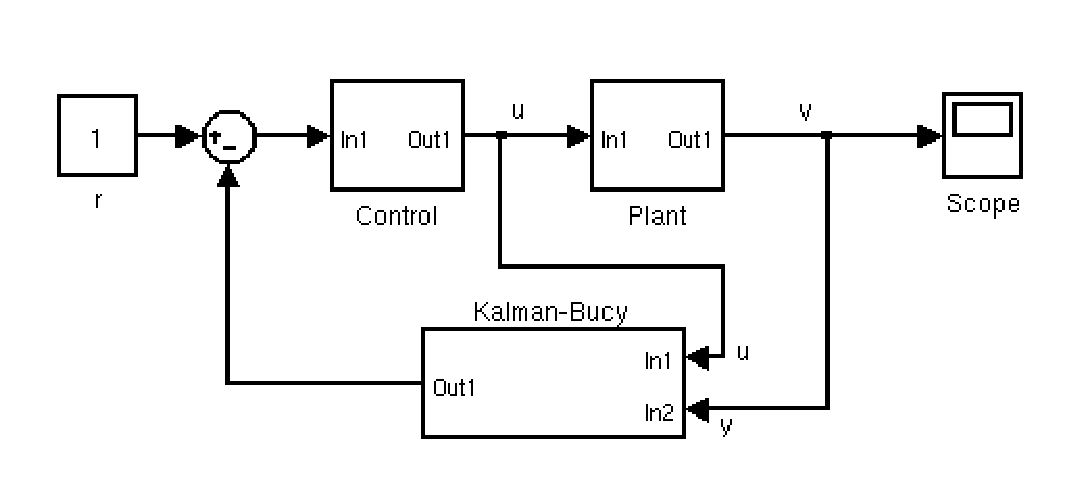
\includegraphics[width=0.90\columnwidth]{figures/kalman_bucy_filter.eps}
	\caption{Realiza��o de estima��o por realimenta��o}
	\label{fig:kalman_bucy_filter}
\end{figure}

Uma outra maneira de realizar este compensador � calculando uma matriz de realimenta��o equivalente
dita $F(s)$ a partir da sa�da $y$ para a entrada $u$. Esta realiza��o � conhecida como
{\it{Realiza��o em cascata}}. Na Figura (\ref{fig:cascade_realization}) � poss�vel observar a 
estrutura desta realiza��o. Se $u=-K_c\hat{x}$ for substitu�do em (\ref{eq:kalman_bucy_state}) 
obtemos (\ref{eq:kalman_bucy_cascade}).

\begin{equation}
	\frac{\mathrm{d} \hat{x}}{\mathrm{d} t}=A\hat{x}+Bu+K_f(y-C\hat{x})
\label{eq:kalman_bucy_state}
\end{equation}

\begin{figure}[htbp]
	\center
	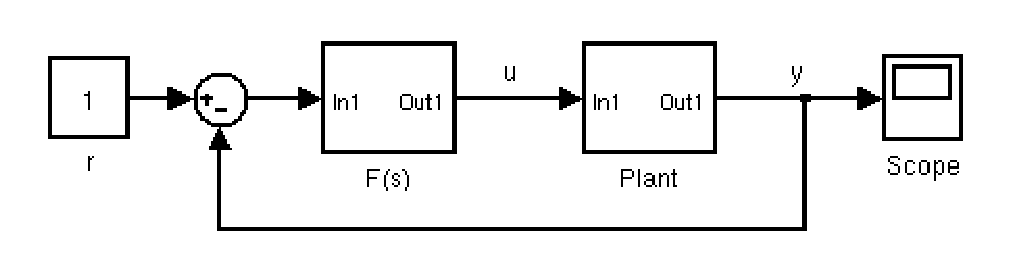
\includegraphics[width=0.90\columnwidth]{figures/cascade_realization.eps}
	\caption{Realizac�o em cascata}
	\label{fig:cascade_realization}
\end{figure}

\begin{equation}
	\frac{\mathrm{d} \hat{x}}{\mathrm{d} t}=(A-BK_c -K_fC)\hat{x}+K_f y
\label{eq:kalman_bucy_cascade}
\end{equation}

A fun��o de transfer�ncia de $y$ para $-u$ pode ser escrita como:

\begin{equation}
	F(s)=K_c(sI-A+BK_c+K_fC)^{-1} K_f\nonumber
\end{equation}

Por conveni�ncia a fun��o transfer�ncia na forma 

\begin{equation}
	F(s)=C_f(sI-A_f)^{-1} B_f+D_f\nonumber
\end{equation}

� escrita:

\begin{equation}
F(s)\equiv \begin{bmatrix}
A_f & B_f\\ 
C_f & D_f
\end{bmatrix}\nonumber
\end{equation}

O espa�o d estado da realiza��o em cascata pode ser escrito como:

\begin{equation}
F(s)\equiv \begin{bmatrix}
A-BK_c-K_fC & K_f \\ 
K_c & 0
\end{bmatrix}\nonumber
\end{equation}

Enquanto que $(A-BK_c)$ e $(A-K_fC)$ s�o ambas matrizes est�veis, a matriz $(A-BK_c-K_fC)$
n�o � necessariamente est�vel, ent�o para alguns tipos de problemas, mesmo com uma
planta est�vel, a realiza��o em cascata ir� requerer um compensador inst�vel. Esta �
a desvantagem da realiza��o em cascata. \cite{lq_control_dorato}

O valor da medida de performance minimo � calculado por:

\begin{equation}
V^{*}=tr\left \{ P K_f \Theta K_f' \right \}+ \left \{ SQ \right \}\nonumber
\end{equation}

Onde $K_f=SC'\Theta^{-1}$ e P satisfaz a Equa��o (\ref{eq:sep_riccati_2}) e S satisfaz
a Equa��o (\ref{eq:sep_riccati_1}).



%===============================================================================
\section{Aplica��es praticas}
\label{sec:applications}

O filtro de Kalman tem uma longa aplicabilidade. Diversas atividades usam ou ate
mesmo dependem dele para seu funcionamento. Abaixo algumas destas aplica��es:

\begin{itemize}
\item Heading Reference Systems
\item Piloto autom�tico
\item estimativa de estado de carga de baterias (SoC)
\item interface c�rebro - computador
\item Sinais Ca�ticos
\item Posicionamento din�mico
\item Economia, em particular macroeconomia, series temporais e econometria
\item sistema de orienta��o por inercia
\item Radar tracker 
\item sistemas de navega��o por sat�lite
\item Localiza��o e mapeamento simult�neos
\item Previs�o do tempo
\item Sistemas de Navega��o
\item Modelagem 3D
\item Vis�o computacional
\item Rob�tica m�vel
\end{itemize}


Nesta sess�o faremos uma pequena introdu��o no que diz respeito a dois destes itens
e uma ideia de como o filtro de Kalman a utilizado. Os t�picos abordados ser�o:
Vis�o computacional (\ref{sec:visao_computacional}) e Rob�tica m�vel (\ref{sec:robotica_movel}).

%===============================================================================
\subsection{Vis�o computacional}
\label{sec:visao_computacional}

Sistemas de vis�o para localiza��o utilizando filtros de Kalman encontram um ponto de aplica��o
bem vasto no quesito de movimenta��o de rob�s em ambientes variados e din�micos.
Existem pesquisas nesta �rea (\cite{zhang_zeng}) para Rob�s moveis aut�nomos 
(autonomous mobile robot -AMR) em ambientes din�micos e incertos. Primeiramente para
obter uma for�a repulsiva aos obst�culos, sonares s�o utilizados para determinar 
o posicionamento dos obst�culos. O Filtro de Kalman a utilizado para eliminar ruido destes
sonares alam do ruido ambiente onde o rob� esta imerso.

Devido aos dist�rbios do ambiente, os sinais do sonar s�o normalmente inst�vel. Para
eliminar os dist�rbios e ru�dos do ambiente � utilizado um filtro de Kalman com 
as seguintes vantagens principais:

\begin{itemize}
\item Sinais de erro de m�nimos quadr�ticos de estima��o s�o obtidos usando computa��o
recursivo, desta forma � r�pido e conveniente para processamento de tempo-real.
\item Um filtro de Kalman est�vel � utilizado para processar sinais inst�veis. Desta
forma o m�todo pode aceitar estes dados dos sonares e garantir uma baixa taxa de ruido.
\cite{zhang_zeng}
\end{itemize}


%===============================================================================
\subsection{Rob�tica M�vel}
\label{sec:robotica_movel}

Um Rob� m�vel pode ser compreendido como rob�s que podem movimentar-se autonomamente
no solo ou no espa�o. Um rob� a um manipulador multifuncional reprogram�vel
projetado para movimentar materiais, ferramentas ou dispositivos especiais
seguindo movimentos programados vari�veis, tendo por objetivo a realiza��o de
tarefas variadas

Para a simula��o do rob� podemos considerar o sistema (\ref{eq:robo_model}). 
\cite{armando_sousa}

\begin{equation}
\frac{\mathrm{d} }{\mathrm{d} t}
\begin{bmatrix}
x(t)\\ 
y(t)\\ 
\theta(t)
\end{bmatrix} = 
\begin{bmatrix}
v(t)cos(\theta(t))\\ 
v(t)sin(\theta(t))\\ 
\omega(t)
\end{bmatrix}
	\label{eq:robo_model}
\end{equation}

Que pode ser melhor entendido pela Figura (\ref{fig:robo_model}).

\begin{figure}[htbp]
	\center
	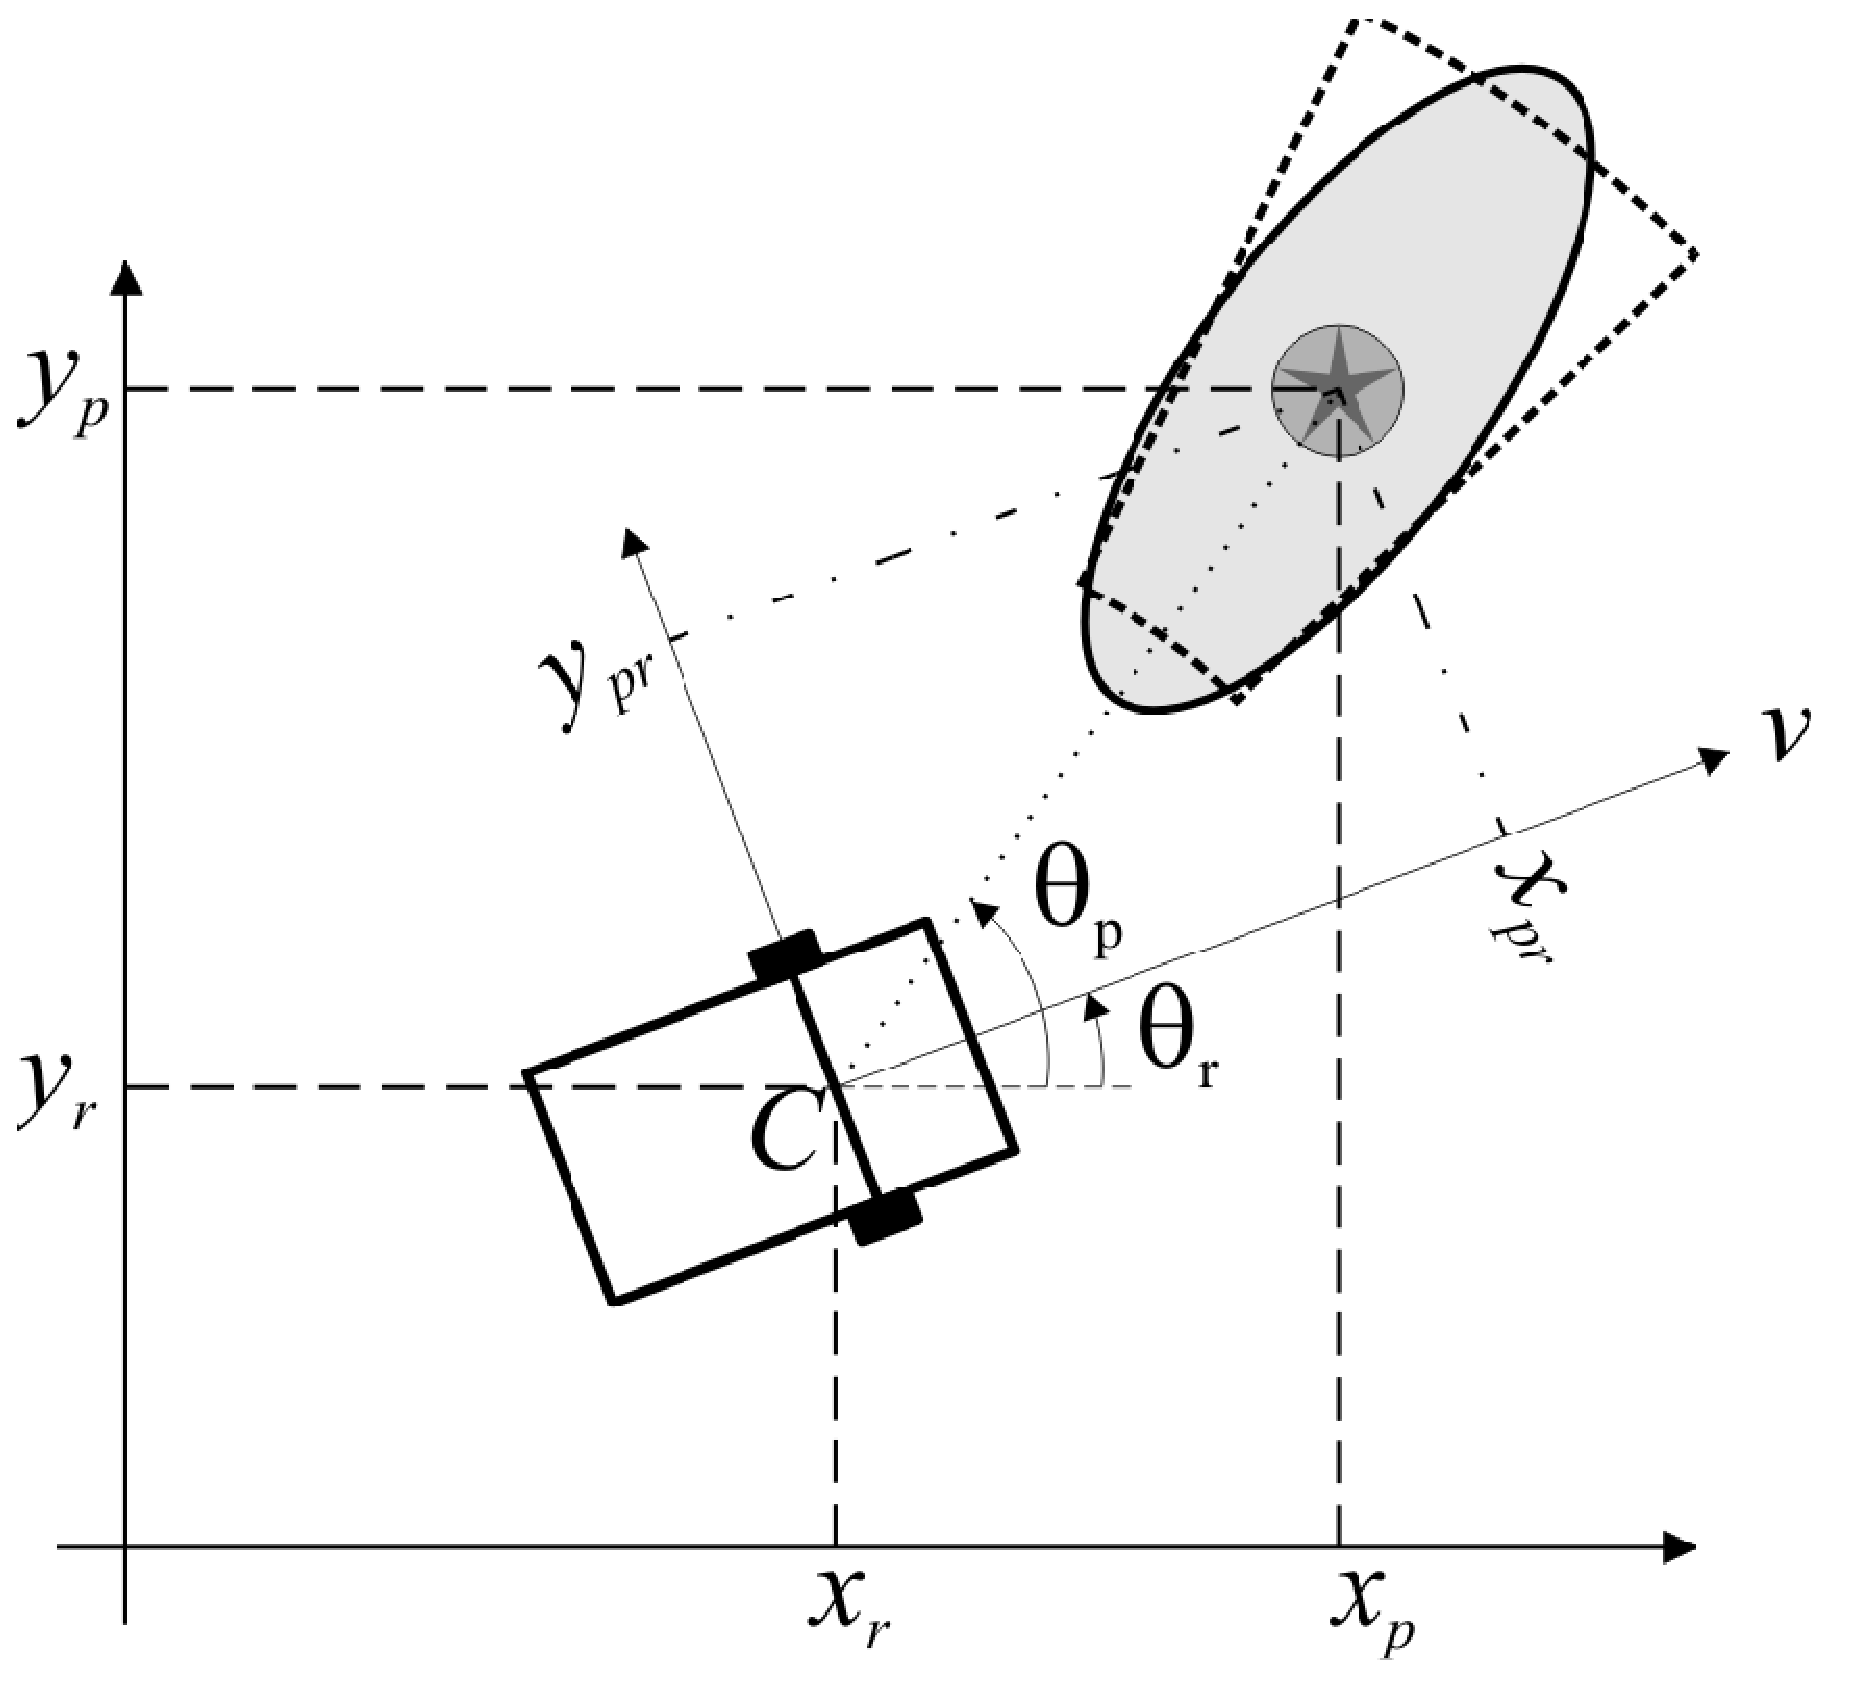
\includegraphics[width=0.80\columnwidth]{figures/robo_model.eps}
	\caption{Representa��o gr�fica do estado do Rob�. \cite{armando_sousa}}
	\label{fig:robo_model}
\end{figure}

Sendo o modelo da cinem�tica do Robot dado pela equa��o (\ref{eq:robo_model})
e considerando-se que os sinais de controle s�o constantes entre cada instante de
amostragem, podemos escrever a equa��o de propaga��o do estado como:

\begin{equation}
\frac{\mathrm{d} X(t)}{\mathrm{d} t}=f(X(t), u(t_k), t) , t \in ]t_k, t_k+1] \nonumber
\end{equation}

Sendo $ u(t)=\begin{bmatrix} v(t) & \omega(t) \end{bmatrix}'$

Desta maneira a poss�vel iniciar o algoritmo do filtro de Kalman. Maiores detalhes podem
ser obtidos em \cite{armando_sousa}.


%===============================================================================
\section{LQR e LQG em tempo discreto}
\label{sec:lqg_lqr}

%===============================================================================
\subsection{LQR para sistemas de tempo discreto}

Para o problema de LQR discreto iremos considerar o valor que o controlador prov�
um valor constante entre duas amostras de tempo ({\it{Zero-order Hold}}). E o sistema
pode ser considerado como em (\ref{eq:lqr_discrate_sys}).\cite{lq_control_dorato}

\begin{equation}
	\dot{x}=\tilde{A}x+\tilde{B}u
	\label{eq:lqr_discrate_sys}
\end{equation}

Usaremos $T$ como o per�odo de amostragem (tempo em que o valor na sa�da do controlador
� mantido constante) e $k$ � um inteiro onde $kT$ ser� o tempo em que o valor continuo
ser� amostrado.

O objetivo do controle discreto � que seja gerada uma entrada $u_k$ tal que o sistema 
em tempo continuo seja minimizado pela performance em (\ref{eq:lqr_v}).

\begin{equation}
V=\int_{t}^{t_f}(x'\tilde{Q}x+u'\tilde{R}u)d\tau+x'(t_f)Sx(t_f)
	\label{eq:lqr_v}
\end{equation}

Temos que:

\begin{equation}
x(t)= \Phi(t,kT)x_k+\int_{kT}^{t}\Phi(t,\tau)\tilde{B}u_k d\tau, \; kT \leq t \leq (k+1)T
	\label{eq:lqr_disc_x}
\end{equation}

\begin{equation}
x_{k+1}=A_k x_k+B_k u_k
	\label{eq:lqr_disc_x}
\end{equation}

Onde:
\begin{equation}
A_k=\Phi((k+1)T, kT)\nonumber
\end{equation}

\begin{equation}
B_k=\int_{kT}^{(k+1)T}\Phi((k+1), \tau)\tilde{B} d\tau \nonumber
\end{equation}

A partir de (\ref{eq:lqr_v}) temos (\ref{eq:lqr_disc}).

\begin{equation}
\int_{kT}^{(k+1)T}(x'\tilde{Q}x+u'\tilde{R}u)d\tau=x_k'Q_k x_k+2u_k'M_k x_k + u_k'R_k u_k
	\label{eq:lqr_disc}
\end{equation}

Onde:

\begin{equation}
Q_k=\int_{kT}^{(k+1)T}\Phi'(\tau, kT)\tilde{Q}\Phi(\tau, kT) \; d\tau
\nonumber
\end{equation}

\begin{equation}
M_k=\int_{kT}^{(k+1)T} H_k'(\tau)\tilde{Q}\Phi(\tau, kT) \; d\tau
\nonumber
\end{equation}

\begin{equation}
R_k=\int_{kT}^{(k+1)T} [\tilde{R}+H_k'(\tau)\tilde{Q}H_k(\tau)] \; d\tau
\nonumber
\end{equation}

\begin{equation}
H_k=\int_{kT}^{\tau}\Phi(\tau, \alpha)\tilde{B} \; d\alpha
\nonumber
\end{equation}

Podemos ent�o re escrever a performance quadr�tica dada em (\ref{eq:lqr_v}) por
(\ref{eq:lqr_v_disc}).

\begin{equation}
V(x_i,i)=\sum_{k=i}^{N-1}l(x_k, u_k, k)\; +x_N'Sx_N
\label{eq:lqr_v_disc}
\end{equation}

Onde $t_f=NT$ e:

\begin{equation}
l(x, u, k)=x'Q_k x + 2u' M_k x + u' R_k u
\nonumber
\end{equation}

%===============================================================================
\subsubsection{Otimiza��o LQR de tempo discreto}

Baseado em (\ref{eq:lqr_v_disc}) e a din�mica descrita em (\ref{eq:lqr_disc_x},
e utilizando o principio da otimalidade temos que o valor �timo para o estado $x_N$
� dado por (\ref{eq:lqr_v_optimal}).\cite{lq_control_dorato}

\begin{equation}
V^{*}(x_N,N)=x_N'Sx_N
\label{eq:lqr_v_optimal}
\end{equation}

O problema a ser minimizado � o apresentado abaixo:

\begin{equation}
\begin{matrix}
x_i'P_i x_i &= \underset{u_i}{min}[x_i'Q x_i+2u_i M x_i+u_i'R u_i \\ 
 & + (Ax_i+Bu_i)' P_{i+1}(Ax_i+Bu_i)
\end{matrix}\nonumber
\end{equation}

Dizemos que o valor de $u_i$ que coloca o sistema no ponto de valor �timo 
� $u_i^* = -K_i x_i$, onde:

\begin{equation}
K_i=(R+B'P_{i+1}A)^{-1}(B'P_{i+1}A+M)
\label{eq:lqr_k_optimal}
\end{equation}

Obtemos ent�o a solu��o da equa��o de Riccati para tempo discreto:

\begin{equation}
\begin{matrix}
P_i= & (Q+A'P_{i+1}A) \\ 
 & -(M+B'P_{i+1}A)'(R+B'P_{i+1}B)^{-1}(M+B'P_{i+1}A)
\end{matrix}
\end{equation}

Onde $P_N=S$.\cite{lq_control_dorato}


%===============================================================================
%\subsection{Problema de filtragem �tima no caso discreto}

%===============================================================================

\section{Conclus�es}
\label{sec:concl}

Foi apresentado neste trabalho uma breve descri��o do funcionamento do
Filtro de Kalman, suas in�meras aplica��es nas mais diversas atividades
e ramos da engenharia moderna. Apresentou-se o diferencial da utilizac�o 
do filtro devido a sua robustez para implementa��o no que diz respeito ao
mundo digital e sua robustez quando existe ruido ou incerteza na planta em
quest�o.

Apresentou-se tamb�m o problema de LQR para tempo discreto, sua modelagem
e a realiza��o do filtro de kalman pelo principio da separa��o, onde a
modelagem do filtro pode ser entendida/resolvida pela resolu��o de um problema
de LQR e outro de LQG.

Apresentou-se tamb�m dois tipos principais para a realiza��o do filtro de kalman:
realiza��o por estima��o (\ref{fig:kalman_bucy_filter}) e a realiza��o em 
cascata (\ref{fig:cascade_realization}).

Com estes pontos apresentados aqui e com a grande aplicabilidade dos filtros
de kalman em problemas comuns da engenharia, observamos que este aparato
tem grande import�ncia e suas aplica��es (\ref{sec:applications}) n�o se 
restringem �s apresentadas neste trabalho.



\bibliographystyle{IEEEtran}
\bibliography{biblio}

\end{document}
